\chapter{Introduction}
\label{chp:Intro}
This thesis document reports on a project undertaken in die biomedical field of wearable electronics. Great advances in miniaturization of electronics and wireless communication have challenged and transformed the norm of the how we use electronics to listen to the language of our bodies: bio-signals. The body constantly gives of signals indicating its physical well-being and the state of its essential physiological functions. Infections are indicated by a rise in core temperature, pneumonia can be detected by a shortness in breath, a abnormal decrease in respiratory rate during sleep can be a warning sign for SIDS, a rise in heart rate can indicate physical stress and abnormal brain activity can be detected at the onset of a seizure. These signals can be detected electronically before observable signs appear. In many cases the deciding factor in the success of a treatment is whether the illness is detected early enough.

\medskip

Because of this, the importance and usefulness of a continuous, wearable health monitor should not be underestimated. Access to accurate, long term data can lead to improved diagnosis of health issues and a better understanding of how our bodies react to drugs, exercise, emotions and the environment around us. Traditionally, bio-signal monitoring is done with a stationary, dedicated device for each signal to be measured. It is easy to see that this is not suitable for continuous and mobile bio-signals monitoring. 

\medskip

This project concerns the design, development and testing of a proof of concept device that will overcome the limitations of these traditional methods. The device is to be worn on the ear like an earphone or hearing aid. I will transmit collected data through a wireless connection to a supporting system for storage and analysis. In this project, the supporting system will be on a laptop, but it can also be on the smart-phone of the wearer or on e cloud server. This supporting system can be used by a physician, caretaker or the wearer self, to monitor and track his/her health.

\medskip

From hear onwards, this device will be referred to as the Ear-Monitor. This report will discuss the project aim and objectives, relevant literature and the design, manufacturing and testing of the Ear-Monitor.

\section{Aim/Research Question}
To develop and test a proof of concept of a wearable device that can monitor bio-signals and transmit collected data wirelessly to a warning and storage system. Bio-signals include core temperature, heart rate, respiratory rate, blood oxygen saturation and electrical brain activity.

\medskip

Is the external ear canal a feasible location for the continuous monitoring of core temperature, heart rate, respiratory rate, blood oxygen saturation and electrical brain activity by means of a ear worn device?

\medskip

In order to achieve the aim of of this project the following three objectives have to be met:
\begin{itemize}
\item Develop an ear worn device to measure core temperature, heart rate, respiratory rate, blood oxygen saturation and electrical brain activity through the external ear.
\item Conduct a trail to determine the functionality of this device.
\item Subsequently, evaluate the feasibility of an ear worm bio-signal monitor
\end{itemize}

\section{Motivation}
This project arose from a need found in medical practise and expressed by the proposer/advocate of this topic. It is the need for better vital sign monitoring methods for neonates and infants in hospital nurseries and a home. High-risk patients are placed in ICUs and are thoroughly monitored, whereas lower risk patients are left in the nursery or sent home. These patients are poorly monitored while at a fragile age, increasing the risk of health issues. This insufficient health monitoring for neonates and infants is due to to the lack of a practical monitoring method. The solution to this issue is the development of a unobtrusive, wearable health monitor.

\medskip

While contemplating and researching this idea, it was found that a much larger group can benefit from such a device. This lead to the project pivoting toward a more general purpose bio-signal monitoring devise. This device will prove if it is practical to measure the mentioned bio-signals through the external ear canal. If this proof of concept is successful, the methods developed during this project can be used to develop specialized ear-worn devices from various applications. In practice, such a device can transmit health statistics and warnings in real time to a physician or caretaker. Applications include:

\begin{itemize}
\item Monitoring neonate- and infant health in nurseries and at home.
\item Monitoring health of patients with chronic illnesses.
\item Studying the effect of prescription drugs or other treatments.
\item Monitoring vital signs and brain activity, like thalamic modulation, of patients during anaesthesia.
\item Monitoring patients with a high seizure/epilepsy risk
\item Monitoring the health of people working under strenuous conditions like heavy machinery operators and soldiers.
\item Tracking the health and fitness of athletes.
\end{itemize}

The ear was chosen as location for the following reasons. The anatomy of the ear and the proximity of an ear-worn device to the tympanic membrane and brain, means that al the bio-signals mentioned can theoretically be measured from this location. This eliminates the need for multiple devices or the need for wires connecting sensors on different parts of the body. The absence of sensors on traditional locations such as the chest or limbs and the absence of connective wires means that the ear-worn device is minimally obstructive for the wearer, especially by freeing up the hands and allowing him/her to move around. The shape of the external ear is ideal for supporting a device without the need for straps or adhesives. Furthermore, the head remains relatively still in relation to the rest of the body. This will reduce the risk of motion artefacts corrupting the signals of interest. An ear-worn device can be embedded in the already familiar shape of a earphone of hearing aid. The final motivation for using the ear as location for the health monitor is its novelty. As will be apparent in the literature review chapter of this document, there is opportunity for research to be done in the unsaturated field of ear-worn health monitors.

\begin{figure}[b]
   \centering
   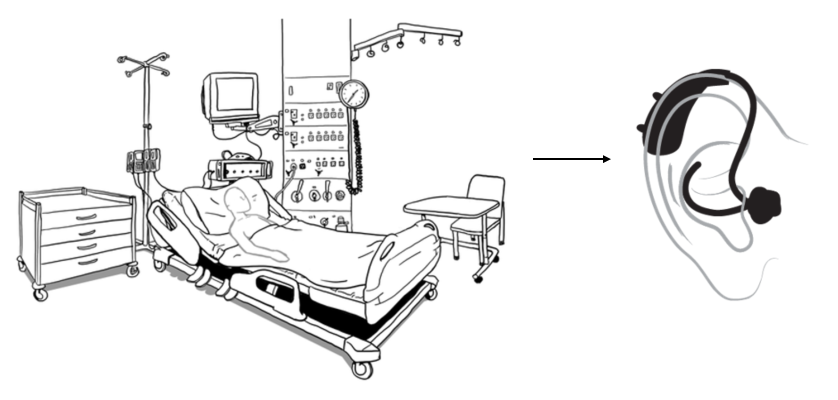
\includegraphics[scale=0.7]{figs/TraditionalICU}
   \caption{Traditional vs.Ear-Monitor (find source)}
   \label{fig:TraditionalICU}
\end{figure}